\chapter{Abi-Training}
\renewcommand{\chaptertitle}{Abi-Training}

\lehead[]{\normalfont\sffamily\hspace*{-2.00cm}\textcolor{white}{\colorbox{lightblue}{\parbox[c][0.70cm][b]{1.60cm}{
\makebox[1.60cm][r]{\thechapter}\\ \makebox[1.60cm][r]{ÜBUNG}}}}\hspace{0.17cm}\textcolor{lightblue}{\chaptertitle}}
\rohead[]{\textcolor{lightblue}{\chaptertitle}\normalfont\sffamily\hspace*{0.17cm}\textcolor{white}{\colorbox{lightblue}{\parbox[c][0.70cm][b]{1.60cm}{\thechapter\\
ÜBUNG}}}\hspace{-2.00cm}}
%\chead[]{}
\rehead[]{\textcolor{lightblue}{AvHG, Inf, My}}
\lohead[]{\textcolor{lightblue}{AvHG, Inf, My}}

\section{Allgemeines}

\subsection{Aufgabe 1: Programmiertechnik}

\begin{compactenum}
\item Wie ruft man Methoden auf, vor denen das Schlüsselwort \lstinline|static|
steht? 
\item Überprüfe mithilfe einer geeigneten Methode, ob in der
\lstinline|char|-Variable \lstinline|c| eine Ziffer (Zahl zwischen \lstinline|0|
und \lstinline|9|) steht.
\item Überprüfe, ob in einer String-Variablen \lstinline|s| die Zeichenkette
\lstinline|"ja"| steht.
\item Schneide die ersten vier Buchstaben aus dem String \lstinline|s| aus.
\item Konvertiere den String \lstinline|s| in eine Integer-Zahl.

Was passiert, wenn s keine Ziffern enthält?
\item Gegeben ist die Variable:	

\lstinline|int i;|

Überprüfe, ob die Zahl \lstinline|i| durch fünf teilbar ist.
\item Konvertiere die Ganzzahl \lstinline|i| in einen String.
\end{compactenum}

\subsection{Aufgabe 2: Netzwerktechnik}

Beantworte folgende Fragen:

\begin{compactenum}
%\item Was ist ein Prozess? Welche Zustände kann ein Prozess annehmen?
\item Was versteht man unter einem Protokoll?
\item Was ist das OSI-Schichten-Modell?
\item Benenne die vier Schichten des vereinfachten Schichten-Modells und erkläre
 ihre Bedeutung.
\item Auf welcher Schicht des OSI-Modells (bzw.\ des Vier-Schichten-Modells)
liegt das IP-Protokoll? Welche Aufgabe hat es?
\item Auf welcher Schicht des OSI-Modells (bzw.\ des Vier-Schichten-Modells)
liegt das TCP-Protokoll? Welche Aufgabe hat es?
\item Auf welcher Schicht des OSI-Modells (bzw.\ des Vier-Schichten-Modells)
liegt das UDP-Protokoll? Welche Aufgabe hat es?
\item Was ist ein DNS-Server?
\end{compactenum}

\subsection{Aufgabe 3: Kryptologie}

Erkläre die folgenden Verfahren und Fachbegriffe:

\begin{compactenum}
\item Caesar-Verschlüsselung
\item Substitutionsverfahren
\item Vigenère-Verfahren
\item Monoalphabetische Verfahren im Vergleich zu polyalphabetischen Verfahren
\item One-Time-Pad
\item DES
\item 3DES
\item AES
\item Symmetrische Verschlüsselung im Vergleich zu asymmetrischer
Verschlüsselung
\item Digitale Signatur
\item RSA
\item Steganographie
\end{compactenum}


\section{Einfache Programmieraufgaben}

\subsection{Aufgabe 1: Satz in Wörter zerlegen}

Schreibe ein Programm, das einen Satz in einzelne Worte zerlegt. 

Das Frame enthält ein Textfeld zur Eingabe des Satzes und einen Button, mit dem
die Berechnung gestartet wird. Wenn der Benutzer auf den Button drückt, wird
der Satz in einzelne Worte zerlegt, die zeilenweise auf der Konsole ausgegeben
werden. Beispiel:

Eingabe:

\myUserInput{In 8 Monaten ist Weihnachten.}

Ausgabe:

\myUserInput{In}\linebreak
\myUserInput{8}\linebreak
\myUserInput{Monaten}\linebreak 
\myUserInput{ist}\linebreak 
\myUserInput{Weihnachten.}

\subsection{Aufgabe 2: Zeichen extrahieren}

Schreibe ein Programm, das einen beliebigen Zeichen aus einem String
herausholt und in einer Messagebox ausgibt.

Das Frame enthält ein Textfeld zur Eingabe einer Zeichenkette und einen Button,
mit dem die Berechnung gestartet wird. Die eingegebene Zeichenkette soll
folgendermaßen aufgebaut sein:

\lstinline|Zahl$Text|

Beispiele:

\bgroup
\def\arraystretch{1.2}
\begin{tabularx}{\textwidth}{p{50mm} X}
Eingabe: \lstinline|1$Abitur| &
Ausgabe: \lstinline|A| \\
Eingabe: \lstinline|12$Abiturvorschlag| &
Ausgabe: \lstinline|h| \\
\end{tabularx}
\egroup

Wenn der Benutzer eine falsche Eingabe macht, soll in einer Messagebox eine
Fehlermeldung ausgegeben werden. Beispiele:

\bgroup
\def\arraystretch{1.2}
\begin{tabularx}{\textwidth}{p{50mm} X}
Eingabe: \lstinline|1Abitur| &
Ausgabe: \lstinline|Das Dollarzeichen fehlt.| \\
Eingabe: \lstinline|$Abiturvorschlag| &
Ausgabe: \lstinline|Die Zeichenkette muss mit einer Zahl beginnen.| \\
Eingabe: \lstinline|10$Abitur| &
Ausgabe: \lstinline|Das angegebene Zeichen existiert nicht.| \\
\end{tabularx}
\egroup

Teste gründlich aus, ob dein Programm bei allen denkbaren Fehleingaben korrekt reagiert.


\section{Q2.2: Client/Server}

\subsection{Aufgabe 1: Dateiinhalte Senden}

Es soll ein Server programmiert werden, der auf Anfrage den Inhalt
verschiedener Dateien an einen oder mehrere Clients sendet. Die Dateien
enthalten eine versteckte Botschaft, die der Server jedoch nur preisgibt, wenn
man zuvor ein geheimes Passwort eingegeben hat.

Zum Testen findest du im Kursverzeichnis ein Client-Programm, mit dem du
beliebige Kommandos an den Server senden kannst. Außerdem gibt es vier
Testdateien, die du in das Verzeichnis deines Servers kopieren solltest.

Der Server soll so programmiert werden, dass er auch mehrere Clients
gleichzeitig bedienen kann. Er wartet auf Verbindungen von Clients auf Port
\lstinline|6666|. Die Oberfläche des Servers kann einfach leer bleiben. Es wird
lediglich die Standard-Funktionalität zum Schließen des Programmfensters
benötigt.

Die Namen der vorhandenen Dateien bestehen aus einem Kleinbuchstaben gefolgt
von der Endung \myFile{*.txt}. Wenn ein Client eine Datei angezeigt bekommen
möchte, sendet er den Kleinbuchstaben, mit dem der Dateiname beginnt, an den
Server. Zum Testen sind nur die Dateien \myFile{a.txt}, \myFile{b.txt} und
\myFile{c.txt} vorhanden. Wenn die gewünschte Datei existiert, schickt der
Server den Inhalt der Datei an den Client und hängt am Ende noch ein
Zeilenumbruch-Zeichen an (\lstinline|'\n'| bzw.\ das ASCII-Zeichen mit dem Code
10). Falls die Datei nicht existiert, sendet der Server den Text 
\lstinline|"Die Datei existiert nicht.\n"| an den Client. Falls ein unerlaubtes
Kommando vom Client kommt (zum Beispiel ein Großbuchstabe), sendet der Server
den Text \lstinline|"Falsche Eingabe\n"|.

Neben dem Senden eines Kleinbuchstaben, gibt es noch drei weitere Kommandos,
die der Client an den Server schicken kann:

\begin{compactitem}
\item \lstinline|$Passwort$| sendet ein Passwort an den Server, mit dem man in
einen Geheimmodus wechseln kann

\item \lstinline|%| schaltet den Geheimmodus wieder aus

\item \lstinline|#Passwort#| ändert das Passwort. Dies geht nur, wenn der
Geheimmodus aktiviert ist.
\end{compactitem}

Wenn der Server das Zeichen \lstinline|'$'| empfängt, weiß er, dass alle
weiteren Buchstaben bis zum nächsten \lstinline|'$'| zu einem Passwort
gehören. Er liest sie ein und vergleicht sie mit dem Text, der in der Datei
\myFile{passwort.txt} steht. Zu Beginn steht in dieser Datei das Passwort
"\lstinline|1234|". Wenn der vom Client empfangene Text mit dem Passwort
identisch ist, schaltet der Server in den Geheimmodus um. An den Client sendet
er die Erfolgsmeldung \lstinline|"Geheimmodus aktiviert\n"|. Falls das Passwort
falsch ist, sendet er \lstinline|"Falsches Passwort\n"| zurück.

Wenn der Server das Zeichen \lstinline|'%'| empfängt, schaltet er den
Geheimmodus wieder aus und sendet den Text 
\lstinline|"Geheimmodus ausgeschaltet\n"| an den Client.

Wenn der Geheimmodus aktiviert ist, wird der Inhalt einer angeforderten Datei
für den Client entschlüsselt und statt des eigentlichen Dateiinhalts das
Geheimwort gesendet, das in dem Text versteckt ist, gefolgt von einem
Zeilenumbruch-Zeichen. Das Geheimwort erhält man, wenn man von jedem Wort den
zweiten Buchstabe nimmt. Alle anderen Buchstaben und Zeichen (Leerzeichen,
Satzzeichen oder Steuerzeichen) werden ignoriert. Wenn das Geheimwort korrekt
entschlüsselt wird, wird aus allen drei Testdateien ein sinnvolles Wort
generiert. Die Datei \myFile{b.txt} enthält zum Beispiel das Geheimwort
\lstinline|abitur|.

Wenn der Server das Zeichen \lstinline|'#'| empfängt, weiß er, dass alle
weiteren Buchstaben bis zum nächsten \lstinline|'#'| zu einem neuen Passwort
gehören. Er liest das neue Passwort ein. Falls der Geheimmodus ausgeschaltet
ist, gibt er die Fehlermeldung \lstinline|"Geheimmodus ist nicht aktiviert\n"|
zurück. Andernfalls schreibt er das neue Passwort in die Datei
\myFile{passwort.txt} und sendet die Erfolgsmeldung 
\lstinline|"Password geändert\n"| an den Client.

Sorge auf geeignete Weise dafür, dass nur ein Client zur Zeit zum Lesen oder
Schreiben auf die Datei \lstinline|passwort.txt| zugreifen kann.


\subsection{Aufgabe 2: Rechentrainer}

Es soll ein Rechentrainer als Client-Server-Anwendung programmiert werden.

\subsubsection{Client}

Erstelle die abgebildete Programmoberfläche. Der untere Button mit der
Aufschrift \myUserInput{Lösung senden} ist zu Beginn deaktiviert. Der obere
Button mit der Aufschrift \myUserInput{starten} ist zu Beginn aktiviert. Das
Textfeld mit der Beschriftung \myUserInput{Aufgabe} ist nicht editierbar.

\begin{center}
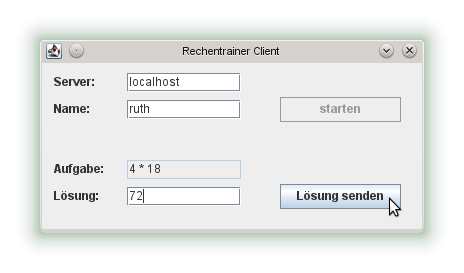
\includegraphics[width=0.7\textwidth]{./inf/SEKII/44_Abi-Training/Rechentrainer.png}
\end{center}

Wenn der Benutzer auf den \myUserInput{starten}-Button drückt, prüft der Client,
ob der Benutzer seinen Namen eingegeben hat. Falls das Namen-Textfeld leer ist,
gibt er eine Fehlermeldung aus. Andernfalls stellt er eine Verbindung zum
Server her, der auf Port \lstinline|33333| wartet. Anschließend sendet er den
Namen des Benutzers an den Server gefolgt von einem \lstinline|$|-Zeichen:

Schema:  \lstinline|Name$|	

Beispiel: \lstinline|Johanna$|

Außerdem deaktiviert er den oberen Button und aktiviert den unteren Button.
Falls die Verbindung zum Server nicht hergestellt werden konnte, wird dem
Benutzer mit \lstinline|JOptionPane.showMessageDialog()| eine Fehlermeldung
ausgegeben.

Wenn der Benutzer auf den unteren Button klickt, wird der Text, den er in das
Lösung-Textfeld geschrieben hat, an den Server gesendet gefolgt von einem
\lstinline|$|-Zeichen:

Schema:  \lstinline|Lösung$|

Beispiel: \lstinline|686$|

Nachdem die Verbindung aufgebaut ist, sendet der Server eine Reihe von
Rechenaufgaben an den Client, die der Client im Aufgaben-Textfeld anzeigt. Eine
Rechenaufgabe kommt in folgendem Format:

Schema: \lstinline|?Aufgabe$|	

Beispiel: \lstinline|?7 * 98$|

Außerdem können vom Server Erfolgs- und Fehlermeldungen kommen. Diese soll der
Client mit Hilfe von\linebreak \lstinline|JOptionPane.showMessageDialog()|
anzeigen:

Schema: \lstinline|%Meldung$|	

Beispiel: \lstinline|%Falsche Antwort. Probier es noch einmal.$|

Der Server stellt dem Benutzer nacheinander fünf Aufgaben (der Client muss dies
nicht mitzählen). Wenn der Benutzer alle Aufgaben erfolgreich gelöst hat,
sendet der Server eine Erfolgsmeldung und schließt dann die Verbindung. Der
Client liest dann entweder eine \lstinline|-1| ein oder erhält beim Lesen eine
Exception. In beiden Situationen soll er als Zeichen für das Ende der Verbindung
den unteren Button deaktivieren und den oberen Button wieder aktivieren. Der
Benutzer kann erneut eine Verbindung zum Server aufbauen, wenn er möchte.

\subsubsection{Server}

Der Server wartet auf Port \lstinline|33333| auf eingehende Verbindungen. Er
kann beliebig viele Clients parallel bedienen. Für die Bearbeitung eines
Clients erzeugt er jeweils einen eigenen Thread.

Nachdem ein Client eine Verbindung zu ihm aufgenommen hat, liest der Server als
erstes den Namen des Benutzers ein, der mit einem \lstinline|$|-Zeichen
beendet wird.

Anschließend stellt er fünf mal hintereinander eine Rechenaufgabe. Dazu
generiert er zwei Zufallszahlen. Die erste Zahl liegt zwischen 2 und 9. Die
zweite Zahl liegt zwischen 10 und 99. Er merkt sich die Lösung der
Rechenaufgabe in einer Variablen und sendet die Aufgabe in folgendem Format an
den Client:

Schema: \lstinline|?zahl1 * zahl2$|	

Beispiel: \lstinline|?7 * 98$|

Dann wartet er auf die Antwort des Clients, die mit einem \lstinline|$|-Zeichen
endet. Er liest die Antwort in eine String-Variable ein und wandelt sie dann in
einen Integer-Wert um. Beachte, dass dabei unter Umständen eine Exception
geworfen wird, falls der Benutzer keine korrekte Zahl angegeben hat. Diese
Exception musst du abfangen, damit in diesem Fall nicht gleich der ganze
Thread beendet wird. Falls das vom Benutzer eingegebene Ergebnis falsch ist,
sendet der Server an den Client zurück:

\lstinline|%Falsche Antwort. Probier es noch einmal.$|

Wenn der Benutzer keine korrekte Antwort gegeben hat, wartet der Server erneut
auf die Antwort des Benutzers und gibt gegebenenfalls wieder die gleiche
Fehlermeldung aus, bis die Antwort richtig ist. Wenn die Antwort korrekt war,
wird sofort die nächste Aufgabe gestellt bis der Benutzer fünf Aufgaben
bearbeitet hat.

Der Server misst die Zeit, die der Benutzer für die Bearbeitung der fünf
Rechenaufgaben benötigt und speichert den aktuellen Bestwert und den Namen des
Benutzers ab, der den Bestwert erzielt hat. Dazu benutzt er folgende Methode
aus der Klasse System:

\begin{lstlisting}
public static long currentTimeMillis()
\end{lstlisting}

Anwendungsbeispiel:

\begin{lstlisting}
long anfangszeit = System.currentTimeMillis();
 ...                                      æ// Berechnung oder ähnliches, deren
æ ...                                      æ// Zeitbedarf ermittelt werden soll
ælong endzeit = System.currentTimeMillis();
double zeit = endzeit - anfangszeit;
zeit = zeit / 1000;                       æ// Umrechnung Millisekunden in Sekunden
\end{lstlisting}

Die Methode gibt die aktuelle Uhrzeit in Millisekunden seit 1970 Millisekunden
zurück (1970 ist sozusagen die Geburtsstunde der Computer). Wenn man die
Methode einmal vor und einmal nach der Bearbeitung der Aufgaben aufruft, kann
man errechnen wie viele Millisekunden der Benutzer zur Bearbeitung der Aufgaben
gebraucht hat. Schreibe das Ergebnis in eine Fließkomma-Variable und rechne den
Wert in Sekunden um. Wenn der Benutzer die Bestzeit erzielt hat, wird an den
Client zurückgegeben:

\lstinline|%Gratuliere Name! Du hast nur Zeit Sekunden gebraucht.\nDas ist die neue Bestzeit!$|

Andernfalls wird zurückgegeben:

\lstinline|%Du hast die Aufgaben in Zeit Sekunden gelöst.\nDie aktuelle Bestzeit von| 
\emph{Name} \lstinline|beträgt|\linebreak \emph{Zeit2} \lstinline|Sekunden.$|

Sorge auf geeignete Weise dafür, dass keine Fehler bei der Speicherung des
Bestwertes und des Benutzernamens entstehen können, weil zwei Clients parallel
zu dem Schluss kommen, dass sie die Besten sind.

Nachdem der Server die Erfolgsmeldung gesendet hat, beendet er die Verbindung
zum Client, indem er den Socket schließt, und beendet auch den Thread, der für
den Client erzeugt wurde. Falls die Verbindung zwischendurch abbricht, zum
Beispiel weil der Benutzer das Client-Programm geschlossen hat, soll der Thread
ebenfalls beendet werden.

Wenn der Client-Thread gestartet wird, liest er die Bestzeit und den Namen des
Benutzers wieder aus einer Datei aus. Speichere die Werte in folgendem Format in
der Datei ab:

Schema: \lstinline|Zeit$Name|	

Beispiel: \lstinline|49.86$Johanna|

Bevor der Client-Thread beendet wird, werden eine möglicherweise verbesserte
Bestzeit und der Name des Benutzers, der die Bestzeit erzielt hat, in der Datei
abgespeichert.

Betrachte den Code des Servers und überlege, an welchen Stellen mehrere Threads
zeitgleich auf dieselben Variablen zugreifen könnten. Schütze diese Bereiche
auf geeignete Weise mit einem Monitor.

\subsubsection{Zusatzaufgabe: UML-Zustandsdiagramm des Servers}

Überlege dir, in welchen Zuständen der Server (es reicht den Client-Thread zu
betrachten) sich befinden kann und bilde die Zustände in einem
UML-Zustandsdiagramm ab.

Versuche anschließend den Client-Thread noch einmal zu programmieren. Und zwar
so, dass der Ablauf über eine Zustandsvariable gesteuert wird. Dabei solltest du
die Zustände benutzen, die du zuvor im UML-Zustandsdiagramm abgebildet hast.


\section{Q2.1: Datenbanken}

\subsection{Aufgabe 1: Osterhasen GmbH}

Die Osterhasen GmbH möchte ihre Verwaltung modernisieren und hat dir einen
Auftrag zur Erstellung einer Datenbank gegeben. Die erfahrene, altgediente
Osterhäsin Emma erklärt dir die Struktur der GmbH:

\begin{quotation}
\noindent
Es gibt verschiedene Lieferbezirke, die jeweils einen bestimmten Stadtteil in
einem Ort umfassen. Wichtig ist dabei die Speicherung der Postleitzahl und des
Stadteilnamens. In jedem Stadtteil gibt es eine ganze Reihe Familien, die
beliefert werden müssen. Einige Familien haben süße Ostereier bestellt, andere
gekochte Eier und viele möchten auch beides haben. Wichtig ist, dass wir von
jeder Familie den Familiennamen wissen sowie die Anzahl der zu beliefernden
Personen und ihre Anschrift (Straße und Hausnummer).

\noindent
Je nach Größe des Lieferbezirks gibt es einen bis maximal fünf Mitarbeiter, die
sich um die Auslieferung unserer Produkte kümmern. Bei besonders kleinen
Bezirken kann es auch mal vorkommen, dass ein Osterhase nicht ausgelastet ist
und gleich mehrere Lieferbezirke bedient. Im Zuge der Emanzipation hat es sich
durchgesetzt, dass nicht nur männliche sondern auch weibliche Osterhasen bei
uns angestellt sind. Wir müssen von jedem Hasen seinen (bzw.\ ihren) Namen und
das Dienstalter wissen.
\end{quotation}

Erstelle zum Entwurf der Datenbank ein geeignetes ER-Diagramm.


\subsection{Aufgabe 2: Schuldatenbank I}

Im Kursverzeichnis findest du die Datei \myFile{schule.sql}, die SQL-Befehle zur
Generierung einer Schuldatenbank erhält. Öffne die Datei als Skript im SQL
Explorer und führe ihre Befehle aus.

\begin{compactenum}[a)]
\item Analysiere die Datenbank und zeichne ein ER-Diagramm, das die Struktur der
Datenbank darstellt.

\item In welcher Normalform befindet sich die Datenbank \myUserInput{schule}?
Begründe deine Antwort, in dem du Schritt für Schritte die Kriterien der
einzelnen Normalformen benennst und überprüfst.

\item Formuliere geeignete Datenbank-Abfragen, mit denen die folgenden
Informationen aus der Datenbank \myUserInput{schule} gewonnen werden können:

\begin{compactenum}[1.]
\item Liste alle Lehrer mit ihren vollständigen Attributen auf. Sortiere die
Lehrer dabei aufsteigend zunächst nach dem Vornamen und dann nach dem Nachnamen.

\item Liste alle Kurse (mit KursId und Fach) auf, die der Lehrer Donald Dusel
 unterrichtet.

\item Erstelle eine Liste mit allen Lehrern (Vor- und Nachname) und den Fächern,
die sie unterrichten. Achte darauf, dass keine Zeilen mehrfach erscheinen.

\item Erstelle für den Schüler Daniel Weber eine Tabelle mit allen seinen
Fächern und der Note, die er jeweils in dem Fach hat. Sortiere die Liste
absteigend nach dem Wert der Note.

\item Liste alle Schüler auf (Vor- und Nachname), die bei der Lehrerin Pia
Bachmann Unterricht haben.

\item Liste alle Schüler auf, die im Fach Mathematik einen Unterkurs haben
(Vorname, Nachname und Note).

\item Ermittle die Anzahl der weiblichen und die Anzahl der männlichen Lehrer.

\item Liste alle Schüler auf (SchülerId, Vorname und Nachname), für die noch
keine Noten eingetragen wurden.

\item Liste alle Fächer auf, für die mehr als ein Kurs angeboten wird (Fach und
 Kursanzahl).

\item Liste alle Lehrer auf (Vor- und Nachname), die mit der Lehrerin Pia
Bachmann ein Unterrichtsfach gemeinsam haben. Frau Bachmann selbst darf auch in
der Liste erscheinen. Es soll jedoch kein Lehrer doppelt aufgelistet werden.
\end{compactenum}

\item Formuliere geeignete Datenbankanweisungen für folgende Datenänderungen:

\begin{compactenum}[1.]
\item Susi Sonntag hat ihren Kollegen Donald Dusel geheiratet und seinen
Nachnamen angenommen. Ändere ihren Nachnamen entsprechend um.

\item Kurs 12 wird von Susi Dusel übernommen. Ändere die LehrerId in der
 Kurs-Tabelle entsprechend.

\item Isabell Steiner verlässt die Schule. Lösche ihren Eintrag in der
 Schüler-Tabelle und alle zugehörigen Einträge in der Noten-Tabelle.

\item Die Schule hat einen neuen Lehrer bekommen. Er heißt Arne Klee. Füge für
Herrn Klee einen neuen Eintrag in die Lehrer-Tabelle ein.
\end{compactenum}
\end{compactenum}


\subsection{Aufgabe 3: Schuldatenbank II}

\begin{center}
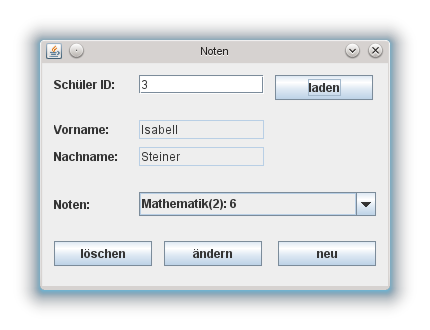
\includegraphics[width=0.45\textwidth]{./inf/SEKII/44_Abi-Training/Noten.png}
\end{center}

Es soll eine grafische Oberfläche für die Schul-Datenbank programmiert werden. Gehe in folgenden Schritten vor:

\begin{compactenum}[a)]
\item Zunächst gibt es im Anwendungsfenster nur drei Textfelder und einen
Button. In das erste Textfeld, das editierbar ist, kann der Benutzer die Id
eines Schülers eingeben. Wenn er auf den Button klickt, schreibt das Programm
den Vor- und Nachnamen des entsprechenden Schülers in die beiden anderen
Textfelder, die nicht editierbar sind. Falls kein Schüler mit der angegebenen
Id existiert, wird in einer Messagebox eine Fehlermeldung ausgegeben.

\item In das Anwendungsfenster wird zusätzlich eine
\myClass{JComboBox}-Komponente eingefügt, in der alle Noten des Schülers nach
folgendem Schema aufgelistet werden:

\lstinline|Fach(Kursnummer): Note|

Beispiel:

\lstinline|Mathematik(2): 13|

\item In das Anwendungsfenster wird zusätzlich ein Button mit der Aufschrift
\myUserInput{Löschen} eingefügt. Wenn der Benutzer den Button anklickt, wird der
vom Benutzer selektierte Eintrag in der \myClass{JComboBox}-Komponente aus der
Tabelle \myUserInput{note} gelöscht (nach einer Sicherheitsabfrage) und die
\myClass{JComboBox}-Komponente wird aktualisiert.

\item In das Anwendungsfenster wird zusätzlich ein Button mit der Aufschrift
\myUserInput{Note ändern} eingefügt. Wenn der Benutzer den Button anklickt, wird
das selektierte Fach aus der \myClass{JComboBox}-Komponente ausgelesen, und der
Benutzer wird nach einer neuen Note für den aktuellen Schüler in dem
selektierten Fach gefragt. Die Note wird in die Datenbank eingetragen und die
\myClass{JComboBox}-Komponente wird aktualisiert.

\item In das Anwendungsfenster wird zusätzlich ein Button mit der Aufschrift
\myUserInput{Neu} eingefügt, mit dem ein neuer Eintrag in die Tabelle
\myUserInput{note} eingefügt werden kann. Wenn der Benutzer den Button anklickt,
wird er in zwei aufeinander folgenden Message-Boxen zunächst nach der KursId und
anschließend nach der Note gefragt. Die eingegebenen Daten werden in die
Datenbank eingefügt und die \myClass{JComboBox}-Komponente wird aktualisiert.
\end{compactenum}


\subsection{Aufgabe 4: Kartenverkauf}

Es soll eine Datenbank für den Kartenverkauf in einem kleinen Theater angelegt
werden. Um in Erfahrung zu bringen, welche Daten abgespeichert werden müssen,
wird die Theaterleitung interviewt, die folgendes berichtet:

\begin{quotation}
\noindent
Das Theater besitzt acht Sitzreihen (durchnummeriert von A bis H) mit je 20
Sitzplätzen (durchnummeriert von 1 bis 20). Pro Tag findet maximal eine
Aufführung statt. Für jede Aufführung müssen das Datum, die Anfangszeit, der
Name des aufgeführten Stücks und der Autor abgespeichert werden. Für jeden
Kunden werden sein Vor- und Nachname, seine Adresse (bitte alle nötigen Details
auflisten) und seine Telefonnummer erfasst. Aus der Datenbank soll ersichtlich
sein, welcher Kunde in welcher Veranstaltung welchen Sitzplatz gebucht hat.
Stammkunden können auch ein Abonnement erwerben. Die Datenbank muss
abspeichern, ob ein Kunde ein Abonnement besitzt oder nicht. Die weitere
Bearbeitung eines Abonnements übernimmt ein Computerprogramm.
\end{quotation}

Entwirf auf Papier ein Entity-Relationship-Diagramm für eine Datenbank, die
alle angegebenen Informationen über die Kunden, die Aufführungen und
vorgenommene Buchungen abspeichern kann. Achte darauf, dass es in der Datenbank
keine Redundanzen gibt.


\subsection{Aufgabe 5: Fahrzeug-Datenbank}

Im Kurs-Repository findest du die Datei \myFile{fahrzeuge.sql}, die SQL-Befehle
zur Generierung einer Fahrzeug-Datenbank enthält. Öffne die Datei als Skript in
im SQL Explorer und führe ihre Befehle aus. Alle weiteren Aufgaben beziehen
sich auf diese Datenbank.

\begin{compactenum}[a)]
\item Untersuche die Datenbank und erstelle ein Entity-Relationship-Diagramm,
das die Struktur der Datenbank beschreibt.

\item In welcher Normalform befindet sich die Datenbank? Begründe deine Antwort.

\item Erstelle geeignete SQL-Abfragen, mit denen die folgenden Informationen
gewonnen werden können.
\begin{compactenum}[1.]
\item Liste alle Fahrzeuge mit ihren (aktuellen und ehemaligen) Fahrzeughaltern
auf. Für die Fahrzeuge sollen das Kennzeichen und der Typ angegeben werden. Für
die Fahrzeughalter werden der Vor- und Nachnamen sowie das Anmelde- und
Abmeldedatum angezeigt. Sortiere die Liste aufsteigend zuerst nach dem
Fahrzeug-Kennzeichen und dann nach dem Anmeldedatum.

\item Erstelle dieselbe Abfrage wie unter 1., aber liste diesmal nur die
Fahrzeughalter auf, die das Fahrzeug aktuell besitzen (d.h.\ die das Fahrzeug
noch nicht abgemeldet haben).

\item Erstelle eine Liste aller Personen aus der Fahrzeughalter-Tabelle mit Vor-
und Nachnamen. In der Liste sollen keine Namen doppelt aufgelistet werden.
Sortiere die Liste absteigend nach dem Nachnamen.

\item Liste alle aktuellen oder ehemaligen Fahrzeuge von Emil Mühltal mit ihren
 vollständigen Fahrzeug-Daten auf.

\item Liste alle Fahrzeuge mit Kennzeichen und Typ auf, die im selben Jahr
gebaut wurden, wie das Fahrzeug \myUserInput{HB - AZ 123}. Das Fahrzeug
\myUserInput{HB - AZ 123} soll nicht in der Liste erscheinen.

\item Erstelle eine Liste aller Fahrzeuge (mit vollständigen Fahrzeug-Daten),
die schon mindestens drei Halter hatten.
\end{compactenum}
\end{compactenum}


\subsection{Aufgabe 6: Fahrzeuge hinzufügen}

Schreibe ein Java-Programm, das ein neues Fahrzeug in die Fahrzeug-Datenbank
einträgt. Bevor der neue Datensatz in die Datenbank eingefügt wird, wird
überprüft, ob bereits ein aktuell angemeldetes Fahrzeug mit dem angegebenen
Kennzeichen existiert. Falls dies der Fall ist wird der Datensatz nicht
eingefügt und stattdessen mit einem \lstinline|showMessageDialog()| eine
Fehlermeldung ausgegeben. Wenn der Datensatz erfolgreich eingefügt wurde, wird
mit einem \lstinline|showMessageDialog()| eine Erfolgsmeldung ausgegeben.

Die Oberfläche des Programms könnte zum Beispiel so aussehen:

\begin{center}
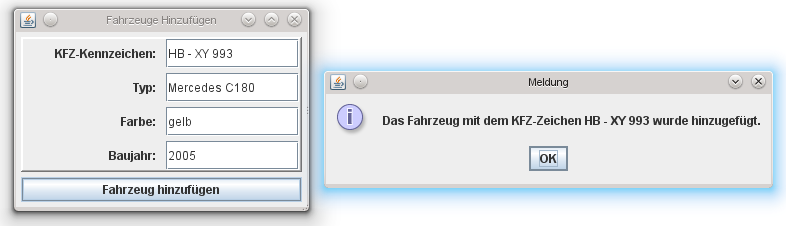
\includegraphics[width=1.0\textwidth]{./inf/SEKII/44_Abi-Training/FahrzeugeHinzufuegen.png}
\end{center}


\subsection{Aufgabe 7: Fahrzeuge abmelden (mit \myClass{JList})}

Erstelle ein Programm mit der abgebildeten Programmoberfläche.

\begin{center}
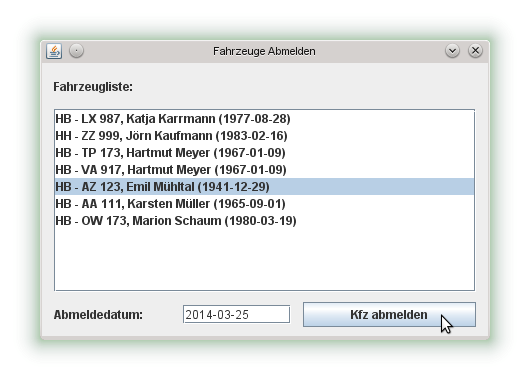
\includegraphics[width=0.7\textwidth]{./inf/SEKII/44_Abi-Training/FahrzeugeAbmeldenMitJList.png}
\end{center}

In der List-Komponente sollen alle Fahrzeuge mit ihren aktuellen
Fahrzeughaltern nach folgendem Schema aufgelistet werden:

\lstinline|KFZ-Zeichen, Vorname Nachname (Geburtstag)|

Als aktuelle Fahrzeughalter werden diejenigen Personen angesehen, bei denen das
Fahrzeug noch nicht abgemeldet ist. 

Wenn man auf den Button abmelden klickt, soll das selektierte Fahrzeug
abgemeldet werden. Dazu trägt das Programm das angegebene Abmeldedatum in den
Datensatz des aktuellen Fahrzeughalters ein. Falls kein Fahrzeug selektiert ist
oder der Benutzer kein Abmeldedatum angegeben hat, werden entsprechende
Fehlermeldungen ausgegeben. Beachte, dass die List-Komponente nach der
Abmeldung eines Fahrzeugs aktualisiert werden muss.


\subsection{Aufgabe 8: Fahrzeuge abmelden (mit \myClass{JComboBox})}

Ändere das Programm aus Aufgabe 6 dahingehend ab, dass statt der
\myClass{JList}-Komponente eine \myClass{JComboBox}-Komponente benutzt wird:

\begin{center}
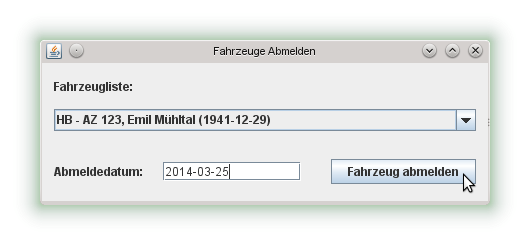
\includegraphics[width=0.7\textwidth]{./inf/SEKII/44_Abi-Training/FahrzeugeAbmeldenMitJComboBox1.png}
\end{center}

\begin{center}
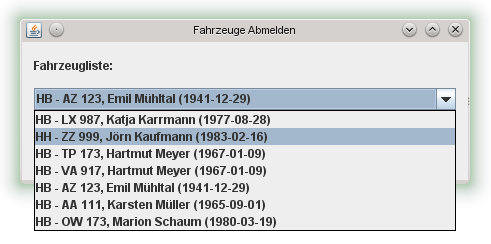
\includegraphics[width=0.65\textwidth]{./inf/SEKII/44_Abi-Training/FahrzeugeAbmeldenMitJComboBox2.png}
\end{center}

An der Programmierung ändert sich dadurch nicht viel:
\myClass{JComboBox}-Komponenten verhalten sich aus Sicht des Programmierers ganz
ähnlich wie \myClass{JList}-Komponenten!


\section{Gemischte Aufgaben (Datenbank plus Client/Server)}

\subsection{Aufgabe 1: Buchhandel}

Es soll der Prototyp für eine Client-Server-Software zum Verkauf von Büchern
erstellt werden. Die Verwaltung der Benutzer wird dabei vernachlässigt. Es wird
für jeden Benutzer einfach eine Benutzernummer eingegeben, ohne den Namen und
die Adresse des Benutzers genauer zu spezifizieren. Auch eine
Zugriffsberechtigung wird nicht abgefragt.

Erzeuge mit Hilfe der Datei \myFile{buchladen.sql} aus dem Kurs-Repository die
Datenbank Buchladen auf deinen Computer.

\subsubsection{ER-Diagramm}

Untersuche die Datenbank und erstelle ein Entity-Relationship-Diagramm, das die
Struktur der Datenbank beschreibt.

\subsubsection{Normalform}

In welcher Normalform befindet sich die Datenbank? Falls sich die Datenbank
noch nicht in der dritten Normalform befindet, gib an, welche Änderungen man
vornehmen müsste, um sie in die dritten Normalform zu bringen.

\subsubsection{Programmierung des Clients}

Programmiere das Client-Programm für den Buchverkauf. 

Im Kurs-Repository findest du einen Server, mit dessen Hilfe du dein Programm
austesten kannst. Erstelle zunächst die Oberfläche des Clients:

\begin{center}
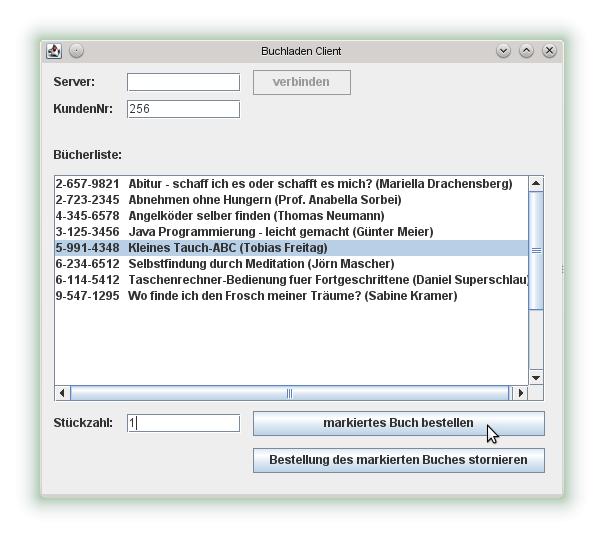
\includegraphics[width=0.85\textwidth]{./inf/SEKII/44_Abi-Training/BuchhandelClient.png}
\end{center}

Zu Beginn soll der verbinden-Button aktiviert sein, und die beiden unteren
Buttons sollen deaktiviert sein. Die Bücherliste soll in einer
\myClass{JList}-Komponente angezeigt werden (nicht in einer
\myClass{JTextArea}).

Wenn der Benutzer auf den verbinden-Button drückt, wird versucht eine
Verbindung zum Server aufzubauen, der auf Port \lstinline|44444| wartet. Falls
der Verbindungsaufbau erfolgreich ist, wird der verbinden-Button deaktiviert
und die beiden unteren Buttons werden aktiviert.

Der Server schickt dem Client sofort eine Liste der vorhandenen Bücher, die der
Client in seiner List-Komponente anzeigen soll. Beachte, dass der Client
zunächst den Inhalt der List-Komponente löschen muss, für den Fall dass sich
dort bereits alte Ausgaben befinden. Die Nachricht des Servers beginnt mit
einem \lstinline|L| (für Liste). Danach wird zeilenweise der fertig aufbereitete
Text für die List-Komponente gesendet. Eine Zeile endet mit einem \textbf{§},
falls noch weitere Zeilen folgen. Die letzte Zeile endet mit einem
\lstinline|$|. Schema:

\lstinline|LZeile|\textbf{§}\lstinline|Zeile|\textbf{§}\lstinline|....|\textbf{§}\lstinline|Zeile$|

Wenn der Benutzer auf den Button \myUserInput{markiertes Buch bestellen} drückt,
prüft der Client, ob der Benutzer in den Textfeldern für die Kundennummer und
Stückzahl einen Inhalt eingegeben hat. Er überprüft auch, ob sich der Eintrag
im Textfeld Stückzahl in eine positive ganze Zahl umwandeln lässt, und ob der
Benutzer in der List-Komponente ein Buch ausgewählt hat. Im Fehlerfall gibt der
Client jeweils mit \lstinline|showMessageDialog()| eine geeignete Fehlermeldung
aus. Wenn alle Eingaben korrekt sind, sendet der Client nach folgendem Schema
eine Bestellung an den Server:

\lstinline|BKundennr$Isbn|\textbf{§}\lstinline|Stückzahl%|

Beispiel: 

\lstinline|B777$5-991-4348|\textbf{§}\lstinline|30%|

Der Server schickt zur Antwort den Buchstaben \lstinline|J| (für Ja), wenn die
Bestellung erfolgreich durchgeführt werden konnte. Falls nicht mehr ausreichend
Bücher vorhanden sind, schickt der Server ein \lstinline|N| (für Nein) gefolgt
von der Anzahl der noch verfügbaren Bücher und einem \lstinline|$|-Zeichen als
Endmarkierung. Der Client muss dem Benutzer in beiden Fällen mit
\lstinline|showMessageDialog()| einen geeigneten Antworttext ausgeben. Beispiel:

\bgroup
\def\arraystretch{1.2}
\begin{tabularx}{\textwidth}{p{30mm} X}
Empfangen: \lstinline|J| &
Ausgabe: \lstinline|Ihre Bücher werden in Kürze versandt.| \\
Empfangen: \lstinline|N30$| &
Ausgabe: \lstinline|Ihre Bestellung kann leider nicht durchgeführt werden.\\n|
\\
& \hspace{15mm}\lstinline|Es sind nur noch 30 Bücher vorhanden.|
\\
\end{tabularx}
\egroup

Wenn der Benutzer auf den Button \myUserInput{Bestellung des markieren Buches
stornieren} drückt, prüft der Client, ob in der List-Komponente ein Buch
markiert ist, und ob die Benutzernummer korrekt eingegeben ist. Falls dies
nicht der Fall ist, gibt er in einem Dialog eine Fehlermeldung aus. Wenn die
Eingaben korrekt sind, fordert er auf folgende Weise vom Server die Stornierung
der Bestellung an:

\bgroup
\def\arraystretch{1.2}
\begin{tabularx}{\textwidth}{p{30mm} X}
\lstinline|SKundennr$Isbn|\textbf{§} &
Beispiel: \lstinline|S777$5-991-4348|\textbf{§} \\
\\
\end{tabularx}
\egroup

Der Server schickt als Antwort den Buchstaben \lstinline|S|, falls die
Stornierung erfolgreich durchgeführt wurde. Falls der Benutzer das markierte
Buch gar nicht bestellt hatte, sendet der Server als Antwort den Buchstaben
\lstinline|F|. Der Client muss in beiden Fällen mit
\lstinline|showMessageDialog()| eine geeignete Meldung an den Benutzer ausgeben.
Beispiel:

\bgroup
\def\arraystretch{1.2}
\begin{tabularx}{\textwidth}{p{30mm} X}
Empfangen: \lstinline|S| &
Ausgabe: \lstinline|Stornierung erfolgreich durchgeführt.| \\
Empfangen: \lstinline|F| &
Ausgabe: \lstinline|Es ist keine Bestellung des markierten Buches vorhanden.|
\\
\end{tabularx}
\egroup

Wenn der Client beim Lesen vom Server eine \lstinline|-1| empfängt oder wenn
ine Exception auftritt, ist die Verbindung zum Server verloren gegangen, weil
der Server gestoppt wurde. In diesem Fall soll der Client seinen Lese-Thread
beenden und die Zustände der Buttons wieder auf den Anfangszustand
zurücksetzen, so dass der Benutzer erneut eine Verbindung zum Server aufbauen
kann, nachdem der Server wieder gestartet wurde. Der
\myUserInput{verbinden}-Button wird dazu wieder aktiviert und die beiden unteren
Buttons werden deaktiviert.


\subsubsection{Programmierung des Servers}

Der Server soll auf Port \lstinline|44444| auf eingehende Verbindungen von
Clients warten. Er soll beliebig viele Clients parallel bedienen können.

Sobald sich ein Client angemeldet hat, liest der Server aus der Datenbank die
Liste aller Bücher aus  und schickt sie an den Client (Schema:
\lstinline|LZeile|\textbf{§}\lstinline|Zeile|\textbf{§}\lstinline|....|\textbf{§}\lstinline|Zeile$|).
Die Buch-Liste soll alphabetisch nach dem Titel sortiert sein. Eine einzelne
Zeile, wird nach folgendem Schema aufgebaut:

\lstinline|ISBN   Titel (Autor)|

Anschließend wartet der Server auf Kommandos, die vom Client gesendet werden.
Wenn eine Buchbestellung vom Client kommt (Schema: 
\lstinline|BKundennr$Isbn|\textbf{§}\lstinline|Stückzahl%|), prüft der Server
zunächst durch eine Datenbankabfrage, ob noch ausreichend Bücher vorhanden
sind. Falls nein, sendet er an den Client die noch vorhandene Anzahl der Bücher
zurück (Schema: \lstinline|NAnzahl$|). Falls ja, speichert er die neue
Bestellung in der Tabelle \myUserInput{bestellung} ab. Außerdem reduziert er in
der Tabelle \myUserInput{buch} die Anzahl der vorhandenen Bücher um die
bestellte Menge. Anschließend sendet er an den Client eine Erfolgsmeldung
(\lstinline|J|)

Wenn eine Stornierung vom Client kommt (Schema:
\lstinline|SKundennr$Isbn|\textbf{§}), bucht der Server alle Bestellungen des
angegebenen Buches für den angegebenen Kunden wieder zurück (Beachte, dass ein
Kunde ein Buch auch mehrere Male bestellen kann!). Dabei muss der Server nicht
nur die entsprechenden Einträge aus der Tabelle \myUserInput{bestellung}
löschen, sondern er muss auch die Anzahl der vorhandenen Bücher in der Tabelle
\myUserInput{buch} um die stornierte Menge erhöhen.

Da der Server mehrere Clients parallel bedienen kann, könnte es passieren, dass
zwei Clients gleichzeitig eine Bestellung oder Stornierung für dasselbe Buch
anfordern. Sorge auf geeignete Weise dafür, dass keine Fehler in der Datenbank
durch parallele Zugriffe auf die Spalte vorhanden in der Tabelle
\myUserInput{buch} entstehen können.
